% Kompiuterijos katedros šablonas
% Template of Department of Computer Science II
% Versija 1.0 2015 m. kovas [ March, 2015]

\documentclass[a4paper,12pt,fleqn]{article}
\usepackage[unicode,colorlinks=false]{hyperref}


\usepackage[utf8x]{inputenc}
%

\usepackage[L7x]{fontenc}
\usepackage{times}
\usepackage{ucs}

 %package to switch the language
\usepackage{etoolbox}

  %set up of the page margins
\usepackage[top=2cm, bottom=2cm, left=3cm, right=1.5cm]{geometry}

 %1.1 line spacing
\linespread{1.1}


  %page numbering at the right side
\usepackage{fancyhdr}
\pagestyle{fancyplain}
\fancyhf{}
\renewcommand{\headrulewidth}{0pt} 
\fancyhfoffset[RO]{0cm}

  %to number at the bottom (exchange lines to number at the top)
\rfoot{\thepage}
  %\rhead{\thepage} %

% \usepackage[usenames,dvipsnames]{pstricks}
\urlstyle{same}
\hypersetup{
%  citecolor=Blue,
%  linkcolor=Blue,
%  urlcolor=Blue
pdfborder={0 0 0 }
}

 %for includegraphics
\usepackage{graphicx}



\usepackage[toc,page]{appendix}


\usepackage{caption}

 %for source codes
\usepackage{listings}
\lstset{commentstyle=\color{red},xleftmargin=10pt, framexleftmargin=6pt, numbersep=1mm, frame=single, numbers=left,numberstyle=\footnotesize,extendedchars=\true, inputencoding=utf8x,basicstyle=\footnotesize,extendedchars=true,
 keywordstyle=\color{black}\bfseries, breaklines=true, breakautoindent=true,framesep=8pt,linewidth=0.95\textwidth
}

 %for algorithms
\usepackage{algorithm}
\usepackage{algorithmic}
 %instead of the above two packages we can use algorithms2e
 %\usepackage[boxed,linesnumbered,vlined,slide]{algorithm2e}

 %special symbols
\usepackage{amsfonts}
\usepackage{amssymb}
\usepackage{amsmath}

 %for theorem like environments
\usepackage{amsthm}

 \usepackage{datetime}
 \renewcommand{\dateseparator}{--}


% SI system units
\usepackage{siunitx}
\sisetup{detect-all}
% Problem with fonts \SI{x.xx}{\micro\metre}, solved with updmap-sys --enable Map=utm.map
\renewcommand{\sfdefault}{uhv}
\renewcommand{\rmdefault}{utm}
\renewcommand{\ttdefault}{ucr}

% List management (itemize, etc.)
\usepackage{enumitem}

\newcommand*{\urlw}[1]{\href{#1}%
            {\nolinkurl{#1}}}

\numberwithin{equation}{section}


\newtoggle{inLithuanian}
 %If the report is in Lithuanian, it is set to true; otherwise, change to false
\settoggle{inLithuanian}{true}

%create file preface.tex for the preface text
%if preface is needed set to true
\newtoggle{needPreface}
\settoggle{needPreface}{false}

\newtoggle{signaturesOnTitlePage}
\settoggle{signaturesOnTitlePage}{true}



\theoremstyle{definition}
\newtheorem{definition}{\keyWordDefinition}
\newtheorem{example}{\keyWordExample}
\def\QED{\unskip\nobreak\hfill\kern5pt$\Box$}

\iftoggle{inLithuanian}{
%\usepackage[L7x]{fontenc}
\usepackage[english,lithuanian]{babel}

\newcommand{\todayiso}{\the\year \dateseparator \twodigit\month \dateseparator \twodigit\day}


\renewcommand{\today}{\number\year\space m. \space \ifcase\month\or
  sausio\or vasario\or kovo\or balandžio\or gegužės\or birželio\or
  liepos\or rugpjūčio\or rugsėjo\or spalio\or lapkričio\or
  gruodžio\fi
  \space\number\day\space d.}


 \usepackage{tocloft}
 \renewcommand\cftsecaftersnum{.} 
 \renewcommand\cftsubsecaftersnum{.} 
 \renewcommand\cftsubsubsecaftersnum{.}

 \usepackage{VUMIFKK}

 \DeclareCaptionLabelFormat{captionlt}{#2 #1}
   %smth is not fine with algorithms 
 \DeclareCaptionLabelFormat{captionltalg}{#2 #1 algoritmas}

 \usepackage{indentfirst}
 \renewcommand{\appendixtocname}{Priedai}
 \renewcommand{\appendixpagename}{Priedai}
 \renewcommand{\contentsname}{Turinys} 

 \renewcommand{\lstlistingname}{išeities kodas}
 \renewcommand{\figurename}{pav}
 \renewcommand{\tablename}{lentelė}


 \captionsetup*[lstlisting]{   
 labelsep=period,labelformat=captionlt
 }
 \captionsetup*[figure]{   
% labelsep=period,
 labelsep=space, %babel redefines pav to pav.
 labelformat=captionlt
 }
 \captionsetup*[table]{   
  labelsep=period,
  labelformat=captionlt
 }
 \renewcommand{\algorithmicrequire}{\textbf{Įvestis:}}
 \renewcommand{\algorithmicensure}{\textbf{Išvestis:}}

 \captionsetup*[algorithm]{   
 labelsep=period,labelformat=captionltalg
 }

\renewcommand{\thmhead}[3]{#2 #1#3}

}
{
%\usepackage[OT1,T1]{fontenc}
%\usepackage[L7x]{fontenc}

\usepackage[english]{babel}
\newcommand{\todayiso}{\twodigit\month \dateseparator \twodigit\day \dateseparator \the\year}
 \captionsetup*[algorithm]{   
 labelsep=period
 }
\captionsetup*[lstlisting]{   
 labelsep=period
 }
 \captionsetup*[figure]{   
 labelsep=period
 }
 \captionsetup*[table]{   
 labelsep=period
 }


}

%some kywords
 \def\keywordAbstract{\iftoggle{inLithuanian}{Santrauka lietuvių kalba}{Abstract}}
 \def\keywordAbstractOther{\iftoggle{inLithuanian}{Santrauka anglų kalba\break(\textit{Summary})}{Santrauka lietuvių kalba}}
 \def\keyWordIntroduction{\iftoggle{inLithuanian}{Įvadas}{Introduction}}
 \def\keyWordConclusions{\iftoggle{inLithuanian}{Rezultatai ir išvados}{Conclusions and Recommendations}}

 \def\keyWordPreface{\iftoggle{inLithuanian}{Pratarmė}{Preface}}
 \def\keyWordAppendice{\iftoggle{inLithuanian}{Priedas}{Appendix}}
 \def\keyWordSignature{\iftoggle{inLithuanian}{parašas}{signature}}
 \def\keyWordDefinition{\iftoggle{inLithuanian}{apibrėžimas}{Definition}}
 \def\keyWordExample{\iftoggle{inLithuanian}{pavyzdys}{Example}}

\newcommand{\bothabstracts}[3]{
\setcounter{secnumdepth}{0}
\newpage
\hspace{2cm}
{\centering{\section{\keywordAbstract}}}

#1
\newpage
\hspace{2cm}
{\centering \section{\keywordAbstractOther}}

\begin{center}{\textbf{#2} }\end{center}

 #3
\setcounter{secnumdepth}{3}
}

 %non-numbered sections: #1 param: for labeling sec:#1, #2 -section title
\newcommand{\sectionWithoutNumber}[2]{\newpage
%\hspace{2cm}
\section*{#1}
\label{sec:#2}
\addcontentsline{toc}{section}{\nameref{sec:#2}}%{#3}
 }



\newcommand{\referenceSources}[1]{
\newpage
\cleardoublepage
\phantomsection
\iftoggle{inLithuanian}{
 \renewcommand{\refname}{Šaltiniai}

 \addcontentsline{toc}{section}{Šaltiniai}
 \markboth{\refname}{Šaltiniai}
 }
{

\addcontentsline{toc}{section}{References}
\markboth{References}{References}
}

\bibliographystyle{plain}
\bibliography{#1}
}



 \newcommand\authorsignature[1]{
\begin{flushright}
 \begin{minipage}[b]{0.45\textwidth}
  \centering
  \rule{\textwidth}{0.5pt}\\
   #1
  \end{minipage}
\end{flushright}
 }




 \newcommand\authorsignatures[5]{%
   \vspace{1cm}
   \authorsignature{#1}
   \ifstrequal{#2}{}{}{\vspace{0.3cm}
     \authorsignature{#2}
     \ifstrequal{#3}{}{}{\vspace{0.3cm}
      \authorsignature{#3}
      \ifstrequal{#4}{}{}{\vspace{0.3cm}
        \authorsignature{#4}
        \ifstrequal{#5}{}{}{\vspace{0.3cm}
         \authorsignature{#5}       
        }
      }
    }
} 
}

\newcommand{\authortitle}{
\iftoggle{signaturesOnTitlePage}{
\tiny{\keyWordSignature}
}{}
}

\newcommand{\depttitlepage}[8]
{
\thispagestyle{empty}
\begin{center}


\includegraphics[width=2cm]{jb_VU_zenklas}

%\vspace{-1cm}

\iftoggle{inLithuanian}
{ 
  VILNIAUS UNIVERSITETAS\\
  MATEMATIKOS IR INFORMATIKOS FAKULTETAS\\
  KOMPIUTERIJOS KATEDRA
}
{
  VILNIUS UNIVERSITY \\
  FACULTY OF MATHEMATICS AND INFORMATICS \\
  DEPARTMENT OF COMPUTER SCIENCE II
}

\vspace{5cm}

#1\\
\vspace{0.5cm}
\textbf{\Large #2}
\end{center}

\vspace{5cm}


\hspace{0.5\textwidth}
\begin{minipage}{0.4\textwidth}
 \begin{flushleft} 
\iftoggle{inLithuanian}
{
 \ifstrequal{#3}{}{}{Atliko:\\[5pt]}
}
{
\ifstrequal{#3}{}{}{Done by:\\[5pt]}
}

%\noindent
\begin{tabular}{@{}lr}%\setlength\tabcolsep{0pt}
\ifstrequal{#3}{}{}{#3&\hspace{2cm}\authortitle\\[5pt]}
\ifstrequal{#4}{}{}{#4&\authortitle\\[5pt]}
\ifstrequal{#5}{}{}{#5&\authortitle\\[5pt]}
\ifstrequal{#6}{}{}{#6&\authortitle\\[5pt]}
\ifstrequal{#7}{}{}{#7&\authortitle\\}
\end{tabular}

\end{flushleft}

\end{minipage}

\vspace{0.5cm}
\hspace{0.5\textwidth}
\begin{minipage}{0.4\textwidth}
 \begin{flushleft} 

\ifstrequal{#8}{}{}
{

\iftoggle{inLithuanian}
{
Vadovas:
}
{
Supervisor:
}

#8

}

\end{flushleft}

\end{minipage}


\vfill

\begin{center}
Vilnius\\
\the\year
\end{center}

\iftoggle{needPreface}{
 \sectionWithoutNumber{\keyWordPreface}{preface}
Pratarmės (Preface) informacija


\iftoggle{inLithuanian}
{
\vspace{\baselineskip}\hfill
\today
}
{
 \vspace{\baselineskip}\hfill \today
}

 \vspace{5cm}

\iftoggle{signaturesOnTitlePage}{}
{
\authorsignatures{#3}{#4}{#5}{#6}{#7}
}
}{}
\newpage
}

\usepackage{color}
\definecolor{todo-background-color}{rgb}{0.7, 0.7, 0.7}
\newcommand{\TODO}[1]{
\colorbox{todo-background-color}{TODO: #1}
}

\usepackage{setspace}
\onehalfspacing

\begin{document}
 % #1 -report type, #2 - title, #3-7 students, #8 - supervisor
 \depttitlepage{Baigiamasis bakalauro darbas}{Duomenų dimensiškumo mažinimas ir klasifikavimas}{Donatas Kučinskas} 
 {}{}{}{}% students 2-5
 {Vytautas Valaitis}

\tableofcontents


%keywords and notations if needed
\sectionWithoutNumber{Sutartinis terminų žodynas}{keywords}{Pateikiamas terminų sąrašas (jei reikia)}

 %both abstracts
\bothabstracts{Santraukos tekstas rašto darbo kalba...}%tex-file of abstract in original language
{Darbo pavadinimas kita kalba} %if work is in LT this title should be in English
{This is a summary in English...}%tex-file of abstract in other language


 %Introduction section: label is sec:intro
\sectionWithoutNumber{\keyWordIntroduction}{intro}
Klasifikavimas - tai dažnai sutinkama užduotis, turintį įvairių sprendimo būdų.
Šios uždavinio tikslas - identifikuoti, kuriai grupei priklauso tiriamas objektas.
Tiriamieji objektai dažniausiai būna vienos rūšies, aprašomi tam tikrais parametrais, o grupės, kuriems jie yra priskiriami - iš anksto žinomos.
Pavyzdžiui, galima klasifikuoti gyvūnus pagal tam tikras jų fizines savybes - kojų ilgį, storį, kitas kūno apimtis, kailio ilgį ir pan.
Natūralu, kad kiekvienas net ir tos pačios rūšies gyvūnas turės šiek tiek kitokius parametrus, tačiau šie parametrai dažniausiai turi įvairius proporcingumus, pagal kuriuos galima bandyti atspėti, kuriai rūšiai tam tikras gyvūnas priklauso.

%TODO: pridėti paaiškinimą, kad dažniausiai turime daug duomenų?

Norint išspręsti konkretų klasifikavimo uždavinį, paprasčiausias sprendimas atrodo galėtų būti šių grupių parametrų ištyrimas - pavyzdžiui, norint mokėti atskirti triušius nuo liūtų turint jų ilgius nėra sunki užduotis.
Tačiau problema kyla, kai atskiriamos klasės yra labai panašios viena į kitą - tokiu atveju pastebėti tam tikrus dėsningumus ir juos sumodeliuoti bei realizuoti ir kur kas sunkiau.
Be to, sprendžiant konkretų klasifikavimo uždavinį, tektų gilintis į klasifikuojamus objektus - pavyzdžiui, norint sukurti tam tikrų kiškių rūšių klasifikavimą, gilios žinios apie šias kiškių rūšių savybes būtų privalomos.





 %the main part
\newpage
\section{Dirbtinių neuronų tinklas}

Dirbtinis neuronų tinklas - tai tarpusavyje susijungusių dirbtinių neuronų tinklas, kurio užduotis yra spręsti tam tikrą užduotį arba užduotis.
Dirbtinis neuronų tinklas gavęs pradinius užduoties duomenis, juos apdoroja ir taip gaunamas tam tikras atsakymas.
Šis atsakymas nebūtinai yra teisingas - neuronų tinklai suprojektuoti taip, kad galėtų būti mokomi kai gauna neteisingą atsakymą.

\subsection{Dirbtinis neuronas}

Dirbinių neuronų tinklas sudarytas iš daugybės dirbtinių neuronų, todėl norint suprasti tinklą, reikia pradėti nuo vieno dirbtinio neurono.
Žmogaus smegenys sudarytos iš daugybės neuronų.
Dirbtinis neuronas - tai supaprastintas šių biologinių neuronų modelis.
Jo modelis pavaizduotas \ref{fig:neuron}~paveiksliuke.
Dirbtinio neurono veikimo principas gan paprastas - per kairėje esančias jungtis dirbtinis neuronas gauna signalus iš kitų dirbtinių neuronų - iš $k$-tosios jungties gaunamas $x_k$ dydžio signalas.
Šiuos signalus neuronas apjungia ir pertvarko, ir taip sugeneruojamas dirbtinio neurono išeinamasis signalas.
Šis išeinamasis signalas gali būti siunčiamas daugybei kitų neuronų - dešinėje esančios jungtys yra neurono išeinamojo signalo jungtys, kuriomis ir yra siunčiamas išeinamasis signalas.

Dirbtinis neuronas generuoja išeinamąjį signalą pagal tam tikrą modelį.
Pirmiausia, kiekviena įeinančioji jungtis turi savo svorį $w_i$ - šis svoris yra padauginamas iš įeinančio signalo dydžio $x_k$.
Tada visos šios signalų dydžių ir svorių sandaugos yra susumuojamos - taip gaunamas skaičius $a$ (\ref{eq:a}~formulė).
Tada šis skaičius $a$ yra paduodamas kaip argumentas tam tikrai funkcijai $f$ ir gaunamas neurono išeities signalas $y = f(a)$.
Šį funkcija $f$ yra vadinama aktyvacijos funkcija - ją galima keisti pagal tai, kokio tikslo siekiama iš šio dirbtinio neurono.
Populiariausios aktyvacijos funkcijos - slenkstinė, tiesinė, hiperbolinis tangentas bei sigmoidinė (\ref{eq:sigmoid}~formulė).
Iš esmės akvyvacijos funkcija gali būti bet kokia funkcija, tačiau vėliau norint apmokyti dirbtinį neuronų tinklą, reikia rasti šios funkcijos išvestinę.
Dėl šios priežasties dažniausiai pasirenkamos tokios aktyvacijos funkcijos, kurios ne tik tinkamai pertvarko signalą išvedimui, tačiau ir kurios išvestinės yra paprastos.

\begin{figure}
	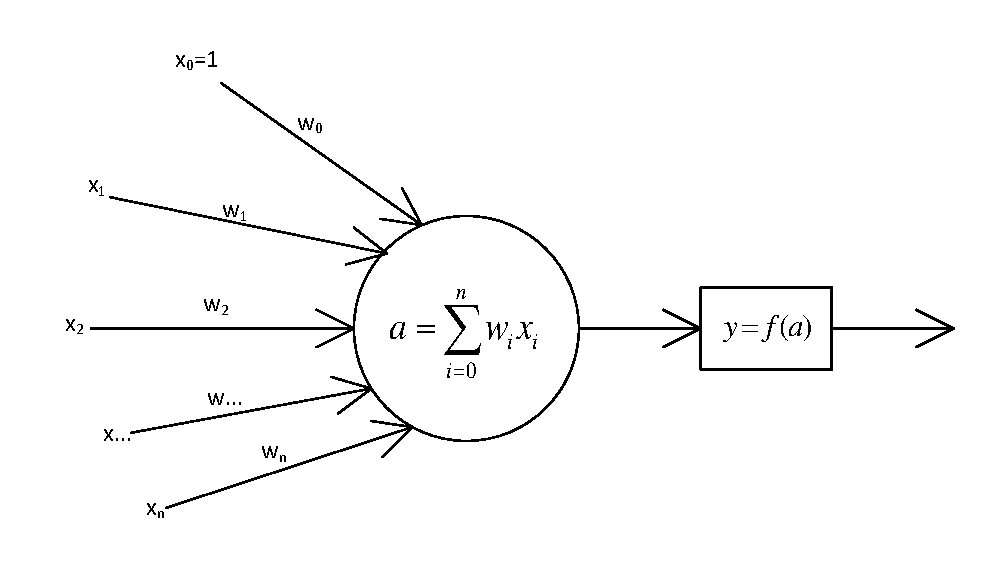
\includegraphics[scale=0.5]{diagrams/1_neuron}
	\caption{Dirbtinis neuronas}
	\label{fig:neuron}
\end{figure}

\begin{equation} \label{eq:a}
a = \sum_{k=1}^N w_kx_k
\end{equation}

\begin{equation} \label{eq:sigmoid}
f(a) = \frac{1}{1 + e^{-a}}
\end{equation}

TODO: bias


\subsection{Dirbtiniai neuronai/tinklas?TODO}

Visi



[TODO: dirbtinio neurono paveiksliukas]


[TODO: citata?]


[TODO: 110 iš knygos]


\section{Dimensiškumo mažinimas}


Klasifikavimo problema

Galimi sprendimai:

	* statistinis sprendimas
	* neuroniniai tinklai
		* veikimas
		* apmokymas
		* validavimas?
		* Klasifikavimas požymių išskyrimui
		* Dimensiškumo mažinimas -> Klasifikavimas

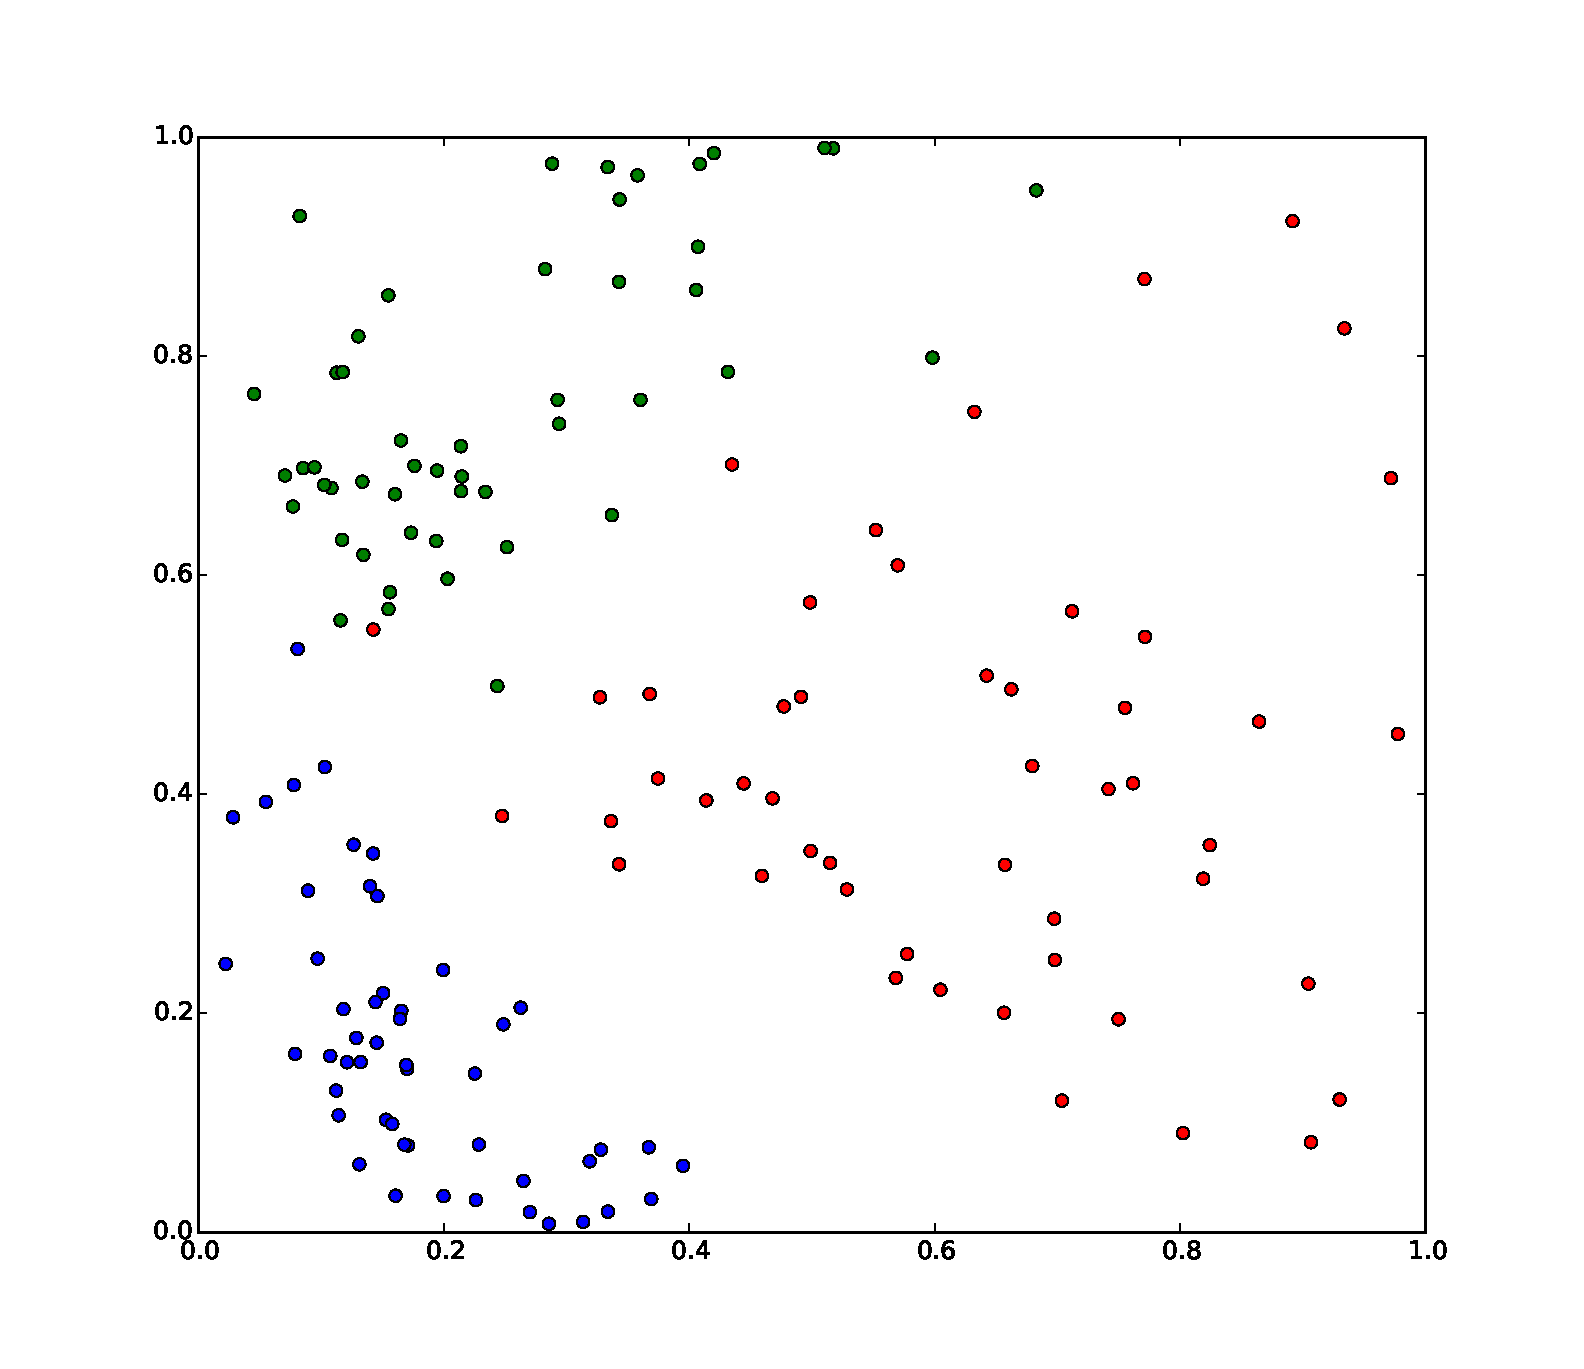
\includegraphics[width=\linewidth]{pics/classification}


\section{Vilkdagių duomenys}

Programuojant neuroninius tinklus, testavimui buvo panaudoti vilkdagių (angl. \textit{Iris flower}) duomenys.
Tai plačiai taikomi ir viešai pasiekiami duomenys, aprašantys 3 rūšių vilkdagius.
Aprašyta po 50 kiekvienos rūšies vilkdagių.
Kiekvienas vilkdagis aprašomas pateikiant 4 dydžius: taurėlapio ilgis, taurėlapio plotis, vainiklapio ilgis bei vainiklapio plotis.
Šiuos vilkdagių duomenis sudaro 150 gėlių, kurių kiekviena aprašyta 4 parametrais bei priskirta vienai iš 3 vilkdagių grupių.

Šie duomenys puikiai tinka klasifikavimo tinklo apmokymui - tinklo tikslas yra kuo mažiau klystant pasakyti, kuriai iš 3 vilkdagių rūšių tam tikra gėlė su tam tikrais parametrais priklauso.
Be to, yra pakankamai duomenų, kad būtų galima dalį jų panaudoti tinklo apmokymui, o kitą dalį - testavimui.
Tokiu būdu bus užtikrinama, kad tinklas teisingai išmoko atskirti vilkdagių rūšis pagal parametrus, o ne tiesiog prisitaikė prie mokymui panaudotų duomenų.

TODO: nuoroda į Vilkdagių duomenis?

Šaltinis ~\cite{KTZ}.

\begin{table}[!ht]\centering
\caption{Lentelė ... }
\label{tabl:table}
\begin{tabular}{l|r|}
test&test\\ \hline
test&test\\
\end{tabular}
\end{table}


 %Conclusions section
\sectionWithoutNumber{\keyWordConclusions}{conclu}
Išvados bei rekomendacijos.


%ateities darbų gairės, planas/next steps of the work
\sectionWithoutNumber{Ateities tyrimų planas}{future}{Pristatomi ateities darbai ir/ar jų planas, gairės tolimesniems darbams....}

 %file literatureSources.bib
\referenceSources{literatureSources}



%% this part is optional
\newpage
\begin{appendices}
Dokumentą sudaro du priedai: \ref{app:a}~priede  ....
\newpage
\section{Pirmojo priedo pavadinimas}
\label{app:a}
Pirmojo priedo tekstas ...

\newpage
\section{Antrojo priedo pavadinimas}
Antrojo priedo tekstas ...

\end{appendices}


\end{document}
